% Build from this directory:
% latex -interaction=nonstopmode -halt-on-error prufer-1.tex
% dvisvgm --no-fonts --exact --bbox=papersize prufer-1.dvi -o prufer-1.svg
\documentclass[tikz,border=5pt]{standalone}
\begin{document}
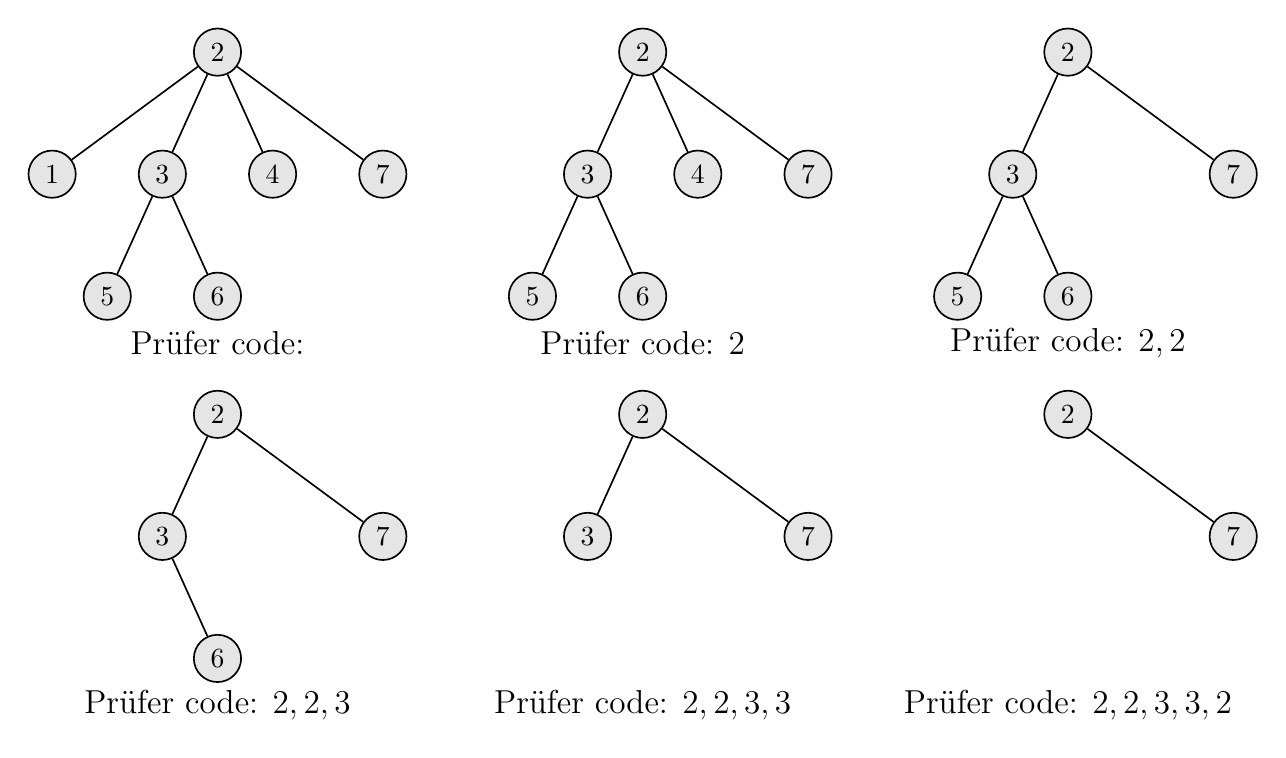
\begin{tikzpicture}[
  vertex/.style={circle,draw,fill=gray!20,minimum size=6mm,
    inner sep=0pt,font=\normalsize},
  line width=.6pt
]
  % All panels use the same positions. Removing the smallest leaf in turn
  % gives 1, 4, 5, 6, 3 and appends its neighbour to the code.
  \newcommand{\pruferpanel}[5]{%
    \begin{scope}[shift={(#1,#2)}]
      \coordinate (p1) at (-2.1,0);
      \coordinate (p2) at (0,1.55);
      \coordinate (p3) at (-.7,0);
      \coordinate (p4) at (.7,0);
      \coordinate (p5) at (-1.4,-1.55);
      \coordinate (p6) at (0,-1.55);
      \coordinate (p7) at (2.1,0);
      \foreach \id in {#3}
        \node[vertex] (n\id) at (p\id) {\id};
      \foreach \from/\to in {#4}
        \draw (n\from) -- (n\to);
      \node[font=\large] at (0,-2.15) {Pr\"ufer code: #5};
    \end{scope}%
  }
  \pruferpanel{0}{0}{1,2,3,4,5,6,7}{1/2,2/3,2/4,2/7,3/5,3/6}{}
  \pruferpanel{5.4}{0}{2,3,4,5,6,7}{2/3,2/4,2/7,3/5,3/6}{$2$}
  \pruferpanel{10.8}{0}{2,3,5,6,7}{2/3,2/7,3/5,3/6}{$2,2$}
  \pruferpanel{0}{-4.6}{2,3,6,7}{2/3,2/7,3/6}{$2,2,3$}
  \pruferpanel{5.4}{-4.6}{2,3,7}{2/3,2/7}{$2,2,3,3$}
  \pruferpanel{10.8}{-4.6}{2,7}{2/7}{$2,2,3,3,2$}
\end{tikzpicture}
\end{document}
